\documentclass[lecture.tex]{subfiles}

\begin{document}

\exercice{Wissam Benmalek}
%\video{https://youtu.be/blablabla}
\enonce{rdm-0019}{Effort et moment résultant d'un système de force}

On considère 3 cas de chargement sur une poutre AC encastrée en A et libre en C (fig.\ref{Poutre_EL}).

\begin{figure}[h]
  \centering
  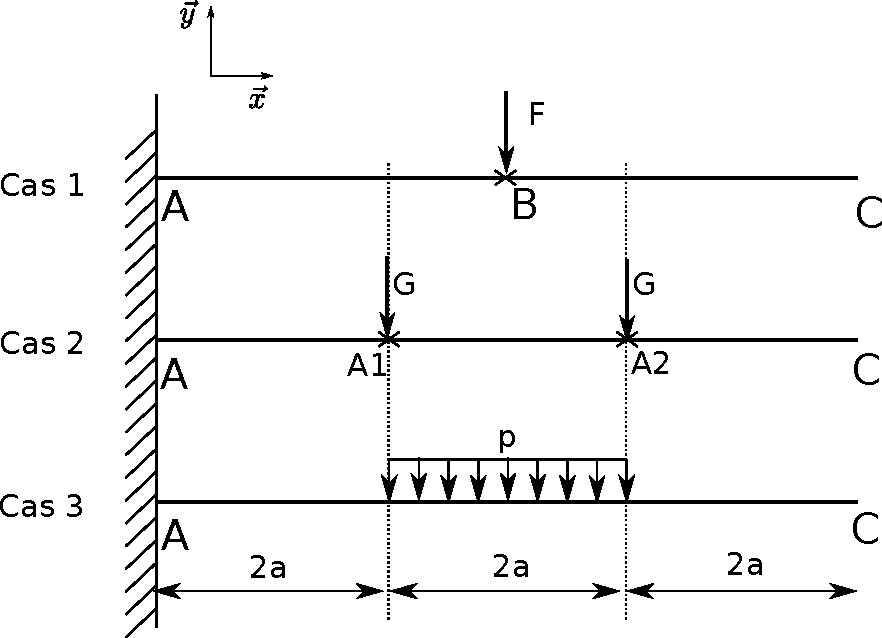
\includegraphics[scale=0.6]{exo1.pdf}
  \caption{Poutre encastrée-libre sous différents chargements}
  \label{Poutre_EL}
\end{figure}

\begin{enumerate}
  \item Calculer les réactions en A dans chacun des cas.
  \item Est-il possible de choisir les données en effort $p$ de manière à ce que chacun des chargement ait un effort et un moment résultants en A identique à celui du premier chargement?
\end{enumerate}

\finenonce{rdm-0019}
\finexercice

\end{document}
